\documentclass[10pt,twocolumn,letterpaper]{article}

\usepackage{times}
\usepackage{graphicx}
\usepackage{float}
\usepackage[italian]{babel}
\usepackage{csvsimple}
\usepackage[shortlabels]{enumitem}
\usepackage{listings}

\begin{document}


\title{Random Maze Solver\\
\large Parallel Programming for Machine Learning}

\author{Sofia Galante\\
\small sofia.galante@stud.unifi.it\\
}
\date{}
\maketitle
\thispagestyle{empty}

\section{Introduzione}

Il programma scritto per questo esperimento è un \textbf{Random Maze Solver}: un labirinto (generato in modo random) viene risolto da delle particelle che si muovono al suo interno, scegliendo il percorso da seguire randomicamente.\\
La particella più veloce (cioè che esce dal labirinto con il minor numero di passi) mostra il cammino corretto da seguire all'interno del labirinto.\\
Si sono creati due diversi \textbf{Random Maze Solver}: uno di tipo sequenziale (in cui cioè le particelle entrano nel labirinto una per volta) e uno di tipo parallelo (in cui più particelle risolvono il labirinto contemporaneamente).\\
\\
Lo scopo di questo elaborato è quello di osservare lo \textit{speedup} ottenuto nel secondo tipo di \textbf{Random Maze Solver} rispetto al primo.\\
Il linguaggio di programmazione utilizzato è il C++ (con compiler MinGW) e la parallelizzazione è stata svolta con \textbf{OpenMP}.\\
\\
Gli esperimenti si sono svolti su un PC con Windows 10 come sistema operativo e una CPU Intel Core i5-11400.

\section{Organizzazione delle classi}
Il codice è composto da 7 classi.

\subsection{La classe \textit{Coordinate} e la classe \textit{Map}}
La classe \textbf{Coordinate} serve a indicare la coordinata di una posizione nel labirinto. Essa permette di settare le coordinate di un punto (con il metodo \textit{setCoordinate()} e di osservare se due punti hanno le stesse coordinate o no (con un override degli operatori \textit{==} e \textit{!=}).\\
\\
La classe \textbf{Map} rappresenta la mappa del labirinto. Essa viene usata dalla classe \textbf{Maze} per definire quali coordinate del labirinto siano muri o meno e quale direzione sia stata presa nella creazione del cammino da una cella all'altra e dalla classa \textbf{Particle} per tenere traccia dei movimenti fatti all'interno del labirinto.

\subsection{La classe \textit{Maze}}
La classe \textbf{Maze} rappresenta il labirinto da risolvere. Quando viene istanziato un oggetto da questa classe, il costruttore procede alla costruzione randomica del labirinto, facendo in modo che esista sempre un cammino valido che vada dall'entrata all'uscita (anche queste sono scelte randomicamente su due mura opposte).\\
I metodi che vengono utilizzati nella creazione del labirinto sono:
\begin{enumerate}
\item{il metodo \textit{createMaze()} che coordina la creazione del labirinto, partendo dalla creazione di un cammino valido e poi riempiendo il resto del labirinto con cammini aggiuntivi;}
\item{i metodi \textit{setStartAndEnd()} e \textit{setStartOrEnd()} che scelgono randomicamente l'entrata e l'uscita del labirinto;}
\item{i metodi \textit{placeWalls()} e \textit{placeWall()} che inseriscono i muri nel labirinto;}
\item{i metodi \textit{validMoves()} e \textit{isPointValid()} che servono a trovare le mosse valide da compiere per continuare a costruire il cammino nel labirinto;}
\item{il metodo \textit{getDirection()} che scrive nella coordinata corrente la direzione da cui è stata scelta quella coordinata;}
\item{il metodo \textit{rewind()} che torna indietro nel cammino se ci si trova in un vicolo cieco, in modo da deviare il percorso per cercare l'uscita;}
\item{il metodo \textit{recovery()} che viene attivato solo nel momento in cui i muri siano stati posizionati in modo tale da rendere impossibile raggiungere l'uscita; in questo caso si riparte dall'uscita e si inizia a creare un cammino per poi abbattere il primo muro che si trova con il metodo \textit{findWallsToRemove()}.}
\end{enumerate}
Durante la creazione del labirinto si decide anche un numero massimo di passi con cui le particelle devono risolverlo.

\subsection{La classe \textit{Particle}}
La classe \textbf{Particle} rappresenta le particelle che devono risolvere il labirinto. Ogni istanza di questa classe mantiene nel suo stato il numero di passi fatti e il percorso intrapreso dall'entrata all'uscita.

\subsection{Le classi \textit{MazeSolver}, \textit{MazeSolverSeq} e \textit{MazeSolverPar}}
La classe \textbf{MazeSolver} contiene al suo interno i metodi che servono a far muovere le particelle nel labirinto. Il MazeSolver tiene traccia della posizione della particella e sceglie quale mossa farle compiere in modo randomico, escludendo le mosse in cui essa andrebbe in una posizione occupata da un muro. Inoltre controlla anche che la particella non superi i numeri di passi massimi per la soluzione del labirinto. Infine stampa a schermo il percorso seguito dalla particella più veloce.\\
Uno dei metodi di questa classe, \textit{solve()}, è un metodo puramente virtuale.\\
\\
Le classe \textbf{MazeSolverSeq} e \textbf{MazeSolverPar} sono classi derivate da \textbf{MazeSolver}. Esse implementano in modo diverso il metodo \textit{solve()} così da crearne una versione sequenziale e una parallela. Questo metodo è responsabile della creazione delle particelle, dell'inizio del loro movimento nel labirinto e della scelta della particella vincitrice (cioè quella che esce più velocemente dal labirinto).\\
La parallelizzazione di questo metodo viene descritta nel dettaglio nella sezione successiva.\\
\\
Si noti che la classe \textbf{MazeSolverPar} crea anche una versione parallela del metodo responsabile per la scelta delle mosse valide. Questa versione prevede l'utilizzo di un \textbf{lock} ed è stata utilizzata per svolgere uno dei test presenti nella sezione 4.

\section{Parallelizzazione compiuta in \textit{MazeSolverPar}}
Il codice di soluzione del labirinto è stato parallelizzato in due punti: nella risoluzione del labirinto da parte delle particelle e nella scelta della particella vincitrice.

\subsection{Parallelizzazione della risoluzione del labirinto da parte delle particelle}
Per parallelizzare la creazione delle particelle e la loro risoluzione del labirinto, è stato utilizzato un \textit{parallel for} che permettesse a ogni thread di generare la particella i-esima e di farla muovere poi all'interno del labirinto.\\
Per fare in modo che le particelle utilizzassero una sequenza randomica per il movimento differente le une dalle altre, si è generato un \textit{seed} per ogni particella. Questi sono stati salvati all'interno di un vettore.\\
Per diminuire il più possibile gli accessi in memoria, le variabili \textbf{numParticles} (numero di particelle da creare), \textbf{seeds} (vettore contenente i seed per la generazione dei numeri random) e \textbf{maze} (il labirinto da risolvere) sono stati marcati come \textit{firstprivate}, in modo tale che ogni thread ottenesse una versione privata della variabile inizializzata al valore scelto prima della parallelizzazione.\\
I thread condividono anche un vettore di particelle \textbf{particles} (marcata come \textit{shared}) in cui inserire le particelle che sono uscite dal labirinto nel numero limite di passi. Visto che questa variabile è condivisa, l'inserimento delle particelle al suo interno è stato indicato come una \textit{sezione critica}.

\subsection{Parallelizzazione della scelta della particella vincitrice}
Per scegliere il vincitore si è compiuta una ricerca della particella con il minor numero di passi in modo parallelo all'interno del vettore \textbf{particles}.\\
Per la parallelizzazione si è utilizzato nuovamente un \textit{parallel for}.\\
Visto che la variabile \textbf{winner} (corrispondente alla particella vincente) è \textit{shared}, il suo accesso in scrittura è stato marcato come \textit{critical} e un \textit{flush} della variabile viene effettuato sia prima della lettura che dopo la scrittura.\\
L'altra variabile utilizzata (\textbf{particles}) è stata invece marcata come \textit{firstprivate}.

\section{Esperimenti svolti e risultati}
Per osservare lo \textit{speedup} ottenuto dalla parallelizzazione del codice si sono compiuti diversi esperimenti.\\
In ognuno di essi si è generato il labirinto e si è fatto risolvere sia da un \textbf{MazeSolverSeq} sia da un \textbf{MazeSolverPar}, mettendone poi a confronto i tempi di esecuzione al variare:
\begin{enumerate}
\item{della dimensione del labirinto;}
\item{del numero di particelle;}
\item{del numero di thread generati nella versione parallela.}
\end{enumerate}
Infine si è anche compiuto un esperimento andando a osservare come l'inserimento di un \textit{lock} rallentasse enormemente l'esecuzione del programma.\\
I risultati sono stati salvati in dei file csv utilizzati poi dal programma \textbf{graphics.py} (in allegato) per generare i grafici qui sotto riportati.

\subsection{Variazione della dimensione del labirinto}

Il primo test svolto osserva come varia il tempo impiegato dai due metodi di risoluzione all'aumentare della dimensione del labirinto.\\
Il valore dei parametri di interesse è:
\begin{enumerate}[-]
\item{numero di particelle = 50;}
\item{numero di thread = 10;}
\item{dimensioni del labirinto che partono da 5x5 e arrivano fino a 100x100.}
\end{enumerate}

\begin{figure}[H]
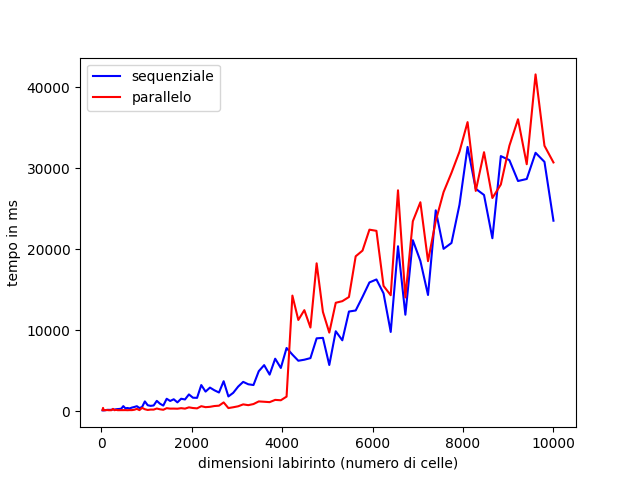
\includegraphics[width=1.1\linewidth]{test/test1}
\caption{\small Tempo impiegato dalla risoluzione sequenziale e dalla risoluzione parallela del labirinto al variare della dimensione (50 particelle).}
\label{t1}
\end{figure}

Questo primo test mostra come l'aumento della dimensione del labirinto possa causare un rallentamento della versione parallela del solver rispetto alla versione sequenziale.

\subsection{Variazione del numero di particelle}

Questo test osserva come variano i tempi all'aumentare del numero di particelle.\\
Il valore dei parametri di interesse è:
\begin{enumerate}[-]
\item{numero di particelle che aumenta da 1 a 1001, muovendosi di 10 in 10 (100 iterazioni in totale);}
\item{numero di thread = 10;}
\item{dimensioni del labirinto = 50x50}
\end{enumerate}

\begin{figure}[H]
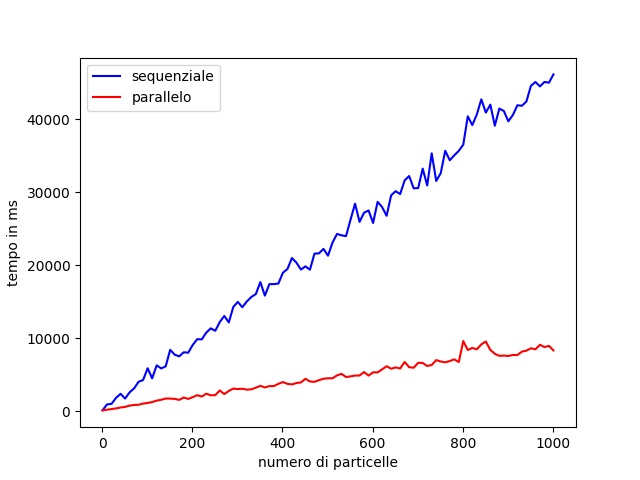
\includegraphics[width=1.1\linewidth]{test/test2}
\caption{\small Tempo impiegato dalla risoluzione sequenziale e dalla risoluzione parallela del labirinto al variare del numero di particelle.}
\label{t2}
\end{figure}

Come si può osservare, maggiore è il numero di particelle, maggiore è la differenza nei tempi di esecuzione del programma.\\
Questo risultato mette in luce quanto l'utilizzo della versione parallela sia utile nel caso in cui ci siano molte particelle da far muovere all'interno del labirinto.

\subsection{Variazione del numero di thread}

In questo test viene variato il numero di thread utilizzati dall'algoritmo parallelo. Si noti che il test sequenziale viene svolto una volta sola, in quanto nessun suo parametro viene modificato.\\
Il valore dei parametri di interesse è:
\begin{enumerate}[-]
\item{numero di particelle = 500;}
\item{numero di thread che aumenta da 1 a 100;}
\item{dimensioni del labirinto = 50x50}
\end{enumerate}

\begin{figure}[H]
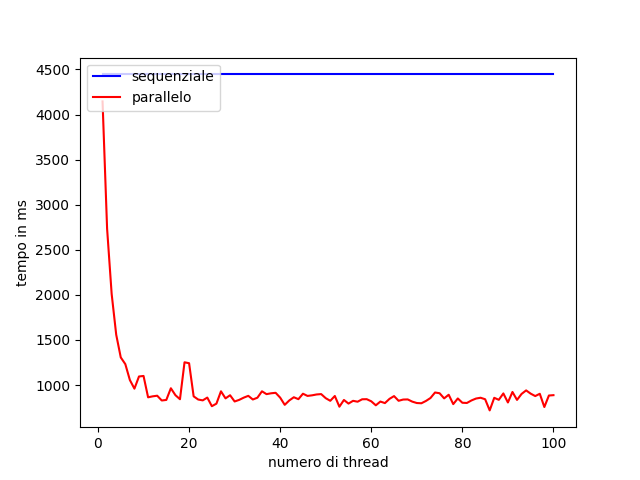
\includegraphics[width=1.1\linewidth]{test/test3}
\caption{\small Tempo impiegato dalla risoluzione sequenziale e dalla risoluzione parallela del labirinto al variare del numero dei thread.}
\label{t3}
\end{figure}

Il risultato di questo test è il più interessante di quelli fino ad ora svolti.\\
Come si può osservare dal grafico, infatti, il metodo parallelo è sempre migliore di quello sequenziale, ma, una volta raggiunto un certo numero di thread, la velocità si stabilizza.\\
Questo fatto mostra come si raggiunga una soglia in cui l'aumento dei thread diventa inutile per la velocizzazione ulteriore del programma: il tempo impiegato a gestire quel numero dei thread è maggiore del tempo guadagnato dalla divisione del lavoro in quegli stessi thread.\\
Per avere un'ulteriore prova di ciò, si è deciso di fare una seconda versione dell'esperimento. In questo caso si è considerato tre diversi risolutori paralleli: il primo solver utilizza 10 thread, il secondo 100 e il terzo 1000.\\
Tutti e tre i solver fanno risolvere un labirinto di dimensioni 50x50 a un numero di particelle variabile da 1 a 1001 (il numero di particelle viene aumentato di 10 in 10, per un totale di 100 iterazioni).\\

\begin{figure}[H]
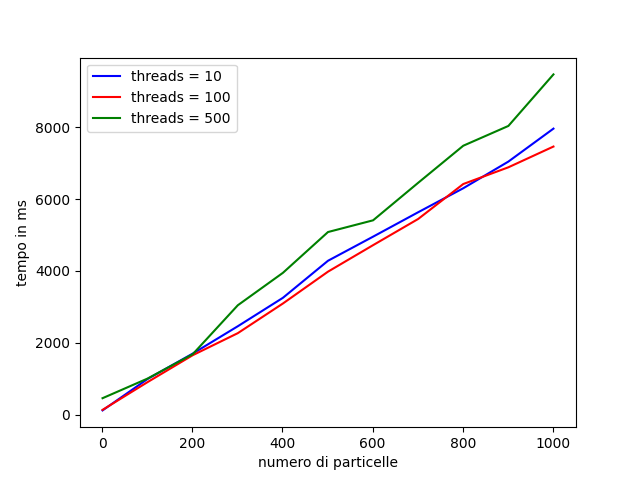
\includegraphics[width=1.1\linewidth]{test/test3_2} 
\caption{\small Tempo impiegato da 3 diverse risoluzioni parallele con diverso numero di thread al variare del numero di particelle.}
\label{t3}
\end{figure}

Il risultato di questo secondo test ci mostra come le supposizioni fatte in quello precedente siano corrette: nonostante le particelle aumentino fino ad arrivare a 1001, il tempo di esecuzione del solver che utilizza 500 thread è molto maggiore dei solver che utilizzano 100 e 10 thread.\\
Inoltre la differenza tra gli altri due solver è molto sottile, dimostrando come anche solo una parallelizzazione compiuta da 10 thread sia sufficiente a ottenere uno \textit{speedup} più che buono.

\subsection{Inserimento del lock}

Questo ultimo test è stato svolto per mostrare come l'inserimento di un lock possa andare a rallentare enormemente il tempo di esecuzione parallelo, rendendolo anche (molto) più lento della versione sequenziale.\\
Il lock in questione è stato inserito nella scelta delle mosse valide per la particella. Ogni volta che il MazeSolver deve scegliere le mosse possibili, infatti, esso controlla se la particella può muoversi nelle quattro direzioni intorno al punto in cui si trova e, se può farlo, inserisce la mossa nel vettore di mosse possibili. Inserendo una parallelizzazione a questo livello, si voleva fare in modo che quattro diversi thread controllassero le quattro mosse.\\
Il lock è stato inserito per la scrittura delle mosse possibili nel vettore.\\
\\
Il risultato dei tempi impiegati è il seguente:
\\
\\
\csvautotabular[separator=semicolon]{test/test4.csv}
\\
\\
\\
Come si può osservare il tempo impiegato dalla versione parallela con il lock non solo è maggiore del tempo parallelo senza lock, ma è nettamente superiore anche al tempo sequenziale.\\
Questa enorme differenza nei tempi è data dalla gestione del lock da parte del sistema che impiega, quindi, un tempo decisamente maggiore di quello guadagnato dalla parellilazione della scelta della mossa possibile.\\
Per questo motivo, il lock deve essere eliminato.
\end{document}
